%% Características del switch principal del GRID

\begin{table}[H]
	\centering
	\sffamily\scriptsize
	\setlength{\tabcolsep}{2pt}
	\renewcommand{\arraystretch}{1.2}
	\caption{Ficha técnica --- Switch Ruijie RG-S5300-24GT4XS-E}\label{table:ruijie-switch}
	\begin{longtable}{|p{0.25\textwidth}|p{0.6\textwidth}|p{0.12\textwidth}|}
		\hline
		\rowcolor{gray!15} \multicolumn{3}{|c|}{\textbf{DESCRIPCIÓN FÍSICA:} Switch administrable de capa 3} \\ \hline

		\textbf{TIPO DE RECURSO:} & Switch Layer 3 administrable &
		\multirow{3}{*}{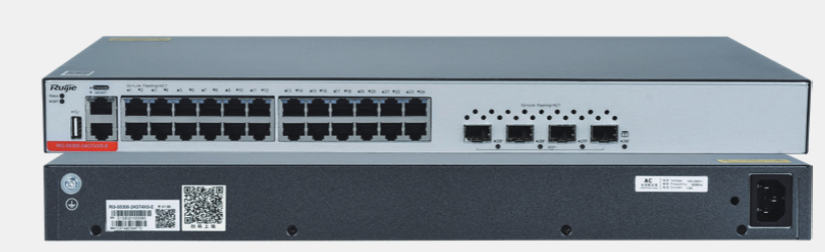
\includegraphics[width=\linewidth,keepaspectratio]{tablas-images/utm/ruiji.png}} \\ \cline{1-2}

		\textbf{MODELO:} & RG-S5300-24GT4XS-E & \\ \cline{1-2}

		\textbf{MARCA:} & Ruijie &
		\\ \hline

		\rowcolor{gray!15} \multicolumn{3}{|c|}{\textbf{FUNCIONALIDADES DE RED Y SEGURIDAD}} \\ \hline

		\textbf{Conectividad} &
		\begin{minipage}[t]{\linewidth}
			• 24 puertos 10/100/1000BASE-T \\ 
			• 4 puertos 1GE/10GE SFP+ \\ 
			• Soporte para enlaces Ethernet Gigabit y 10 Gigabit
		\end{minipage} & \\ \hline

		\textbf{Administración} &
		\begin{minipage}[t]{\linewidth}
			• Puerto RJ45 Console \\ 
			• Puerto RJ45 MGMT \\ 
			• Puerto USB 2.0 \\ 
			• LEDs de monitoreo y estado
		\end{minipage} & \\ \hline

		\textbf{Transmisión soportada} &
		\begin{minipage}[t]{\linewidth}
			• 1000BASE-SX/LX/LH/ZX \\ 
			• 10GBASE-SR/LR/ER/ZR \\ 
			• Cable AOC SFP+ activo
		\end{minipage} & \\ \hline

		\rowcolor{gray!15} \multicolumn{3}{|c|}{\textbf{ESPECIFICACIONES TÉCNICAS}} \\ \hline

		\textbf{CPU} & Procesador Dual-Core de 1.2 GHz & \\ \hline
		\textbf{Memoria RAM} & 1 GB & \\ \hline
		\textbf{Memoria Flash} & 2 GB & \\ \hline
		\textbf{BootROM} & 16 MB & \\ \hline
		\textbf{RTC} & Soportado & \\ \hline
		\textbf{Consumo máximo} & 40 W & \\ \hline
		\textbf{Fuente de alimentación} & Fuente fija AC integrada & \\ \hline
		\textbf{Voltaje de entrada} & 100 V AC a 240 V AC, 50/60 Hz & \\ \hline

		\rowcolor{gray!15} \multicolumn{3}{|c|}{\textbf{CAPACIDADES FÍSICAS}} \\ \hline

		\textbf{Dimensiones} &
		442 mm × 220 mm × 43.6 mm &
		\\ \hline

		\textbf{Formato} &
		1 RU para rack &
		\\ \hline

		\textbf{Peso} &
		2.7 kg &
		\\ \hline

		\textbf{Ventilación} &
		Flujo de aire izquierda-derecha y frontal-derecha &
		\\ \hline

		\textbf{Ventilador} &
		1 módulo de ventilación fijo &
		\\ \hline

		\textbf{Ruido acústico} &
		40.9 dB a 27°C / 48.8 dB a 45°C &
		\\ \hline

		\rowcolor{gray!15} \multicolumn{3}{|c|}{\textbf{CONDICIONES OPERATIVAS}} \\ \hline

		\textbf{Temperatura operativa} &
		0°C a 45°C &
		\\ \hline

		\textbf{Temperatura de almacenamiento} &
		-40°C a 70°C &
		\\ \hline

		\textbf{Humedad operativa} &
		10\% a 90\% RH sin condensación &
		\\ \hline

		\textbf{Altitud operativa} &
		-500 m a 5000 m &
		\\ \hline

		\textbf{MTBF} &
		200,000 horas aproximadamente &
		\\ \hline

		\rowcolor{gray!15} \multicolumn{3}{|c|}{\textbf{CUMPLIMIENTO Y SOPORTE}} \\ \hline

		\textbf{Normativa de seguridad} &
		IEC 62368-1 &
		\\ \hline

		\textbf{Compatibilidad EMC} &
		EN 300386, EN 55032, EN 55035, IEC 61000 &
		\\ \hline

		\textbf{RoHS} &
		Directiva Europea 2011/65/EU &
		\\ \hline

		\textbf{Hot Swap} &
		Soporte para USB y cables intercambiables en caliente &
		\\ \hline

		\rowcolor{gray!15} \multicolumn{3}{|l|}{\textbf{PROPÓSITO:} Gestión y distribución del tráfico de red dentro de la infraestructura del \GRID} \\ \hline

		\rowcolor{gray!15} \multicolumn{3}{|l|}{\textbf{OPORTUNIDAD DE USO:} Segmentación y administración de conectividad en entornos cloud e institucionales} \\ \hline

		\multicolumn{3}{|p{0.97\textwidth}|}{
			\textbf{OBSERVACIONES:} Switch administrable de capa 3 utilizado para la conectividad de la infraestructura del grupo \GRID, permitiendo interoperabilidad con servicios de virtualización, monitoreo y seguridad perimetral.
		} \\ \hline

	\end{longtable}
\end{table}
